\chapter{A Template struktúra}
\label{chap:fejezet4}

Egy webes alkalmazásnak a Template a leglátványosabb része, hiszen ez jeleníti meg a felhasználó számára a kezelőfelületet és animációkat. A Django támogatja a HTML Template-ek öröklődését, ami azért hasznos, mert ezzel sokkal átláthatóbb, és könnyebben karbantartható webalkalmazást kapunk. Az öröklődéshez először is szükség van egy "fő" HTML oldalra, amiből származtatni fogjuk a többit. Erre az oldalra importálhatjuk a CSS és JS fájlokat, amik az egész alkalmazás stílusát és animációit állítják be. Továbbá a navigációs sávot, a fejlécet és a láblécet is itt érdemes megadni. Amikor a fő oldallal készen vagyunk akkor származtathatunk belőle, és minden származtatott oldal megkapja a szülő oldal tulajdonságait. A származtatást úgy oldhatjuk meg, hogy a származtatott oldal elejére az alábbi kódot írjuk:\\

\begin{verbatim}

\end{verbatim}

Ezzel az új html oldalunk szülője a base.html lett. A szakdolgozatomban a base.html oldalt készítettem el a "fő" HTML fájlnak. Ebbe írtam meg a fejlécet, az importokat, a navigációs sávot, és a láblécet. Meg kellett adnom azokat a részeket az oldalon, amiket a belőle származó HTML oldalak változtatni fognak.

\begin{figure}[!htbp]
	\caption{Példa az öröklődésben használt block-okra}
	\label{fig:htmloroklodes}
	\centering
	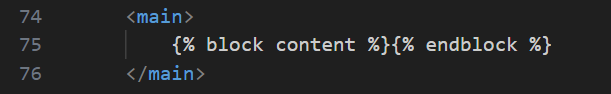
\includegraphics[width=1.0\textwidth]{base_blocks_example.png}
\end{figure}

Az 4.1. ábrán egy példa látható az oldal main részének a block-jára. Ezután, ha írni szeretnénk egy származtatott oldalon ebbe a block-ba, akkor a "content" nevű block-ba szánt kódot\verb|| és \verb|$| kód között kell megadnunk. Ennek hatására a származtatott oldalon megadott block kódot a base.html oldal main részébe fogja helyezni.

\begin{figure}[!htbp]
	\caption{A navigációs sáv kódja}
	\label{fig:navigationbar}
	\centering
	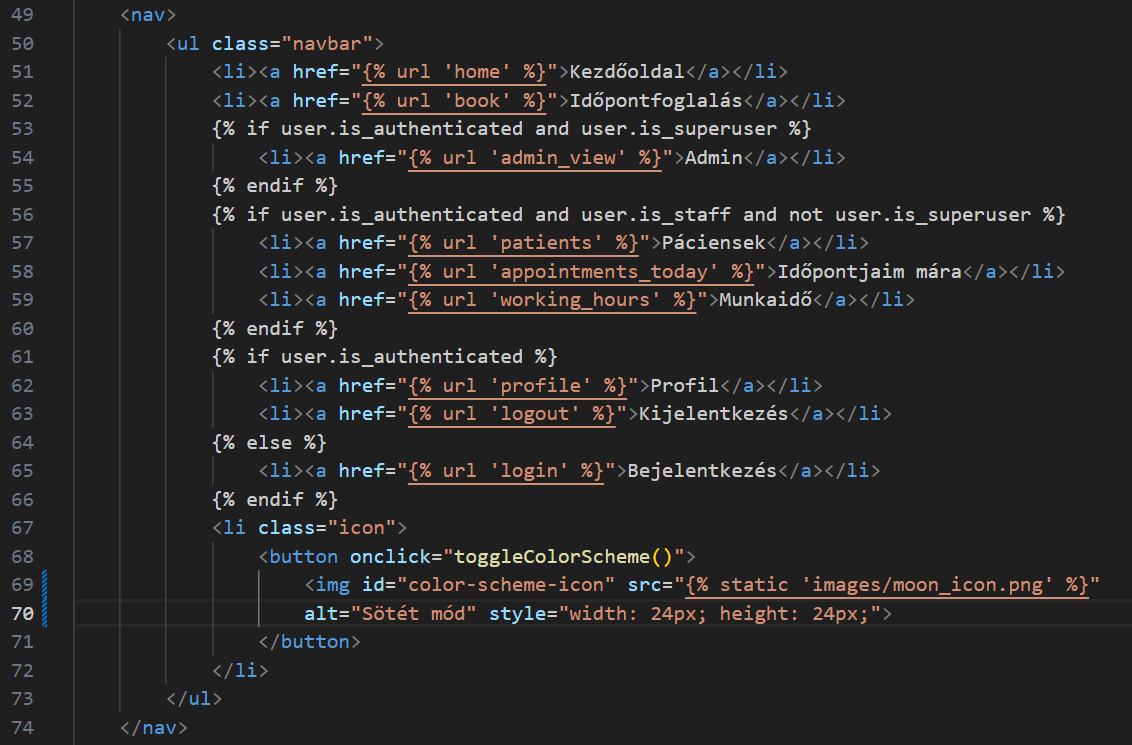
\includegraphics[width=1.0\textwidth]{navbar_code.png}
\end{figure}

A navigációs sáv kulcsfontosságú szerepet tölt be az alkalmazás felhasználhatóságában. A szakdolgozatomban az 4.2. ábrán látható módon oldottam meg a navigációs sáv implementációját a base.html fájlban. Az urls.py fájlban található linkeket adtam hozzá a Django sablonnyelvben írt feltételekkel, hogy a különböző jogokkal rendelkező felhasználók csak a nekik szánt oldalakat láthassák rajta. Ezek a linkek az alkalmazás tobábbi felhasználói felületeire navigálják a felasználót. Ezeken felül pedig van egy gomb is a navigációs sávon, ami a sötét, és világos módok közötti váltást teszi lehetővé egy JS kód segítségével, amire még a későbbiekben kitérek.


